%!TEX root = ../problems.tex
\begin{task}
	Найти и нарисовать амплитудно-частотную характеристику (АЧХ) для цепи, изображённой на рисунке. 
\end{task}
\begin{figure}[h!]
	\centering
	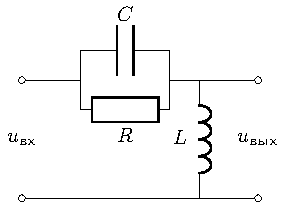
\includegraphics[scale=1.2]{chem/task7}
	\caption{}
	\label{fig:7}
\end{figure}
\begin{gather*}
	\hat{z_\text{экв}}=\frac{\hat{z_R} \cdot \hat{z_C}}{\hat{z_R} + \hat{z_C}}=\frac{R \cdot \frac{1}{j\omega C}}{R + \frac{1}{j\omega C}}=\frac{R}{1+j\omega CR}=\frac{R(1-j\omega CR)}{1+(\omega CR)^2}=\frac{R-j\omega CR^2}{1+(\omega CR)^2}
\end{gather*}
\begin{gather*}
	\hat{K}_\text{экв}=\frac{\hat{U}_\out}{\hat{U}_\in}=\frac{\hat{I} \cdot \hat{z_L}}{\hat{I} \cdot (\hat{z_L}+\hat{z_\text{экв}})}=\frac{\hat{z_L}}{(\hat{z_L}+\hat{z_\text{экв}})}=\frac{j\omega L}{j\omega L+\frac{R}{1+j\omega CR}}=\\=\frac{j\omega L(1+j\omega CR)}{R+j\omega L(1+j\omega CR)}=\frac{j\omega L-\omega^2LCR}{R-\omega^2LCR+j\omega L}
\end{gather*}
\begin{figure}[h!]
	\centering
	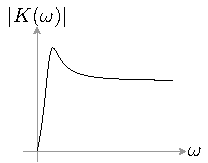
\includegraphics[scale=1.2]{ris/task7_out2}
	\caption{Коэффициент передачи}
	\label{fig:7.1}
\end{figure}
\begin{gather*}
	|\hat{K}_\text{экв}|=\frac{\sqrt{(\omega^2LRC)^2+(\omega L)^2}}{\sqrt(R-\omega^2LRC)^2+(\omega L)^2}=\frac{\sqrt{(RLC)^2+\frac{L^2}{\omega^2}}}{\sqrt{(\frac{R}{\omega^2}-RLC)^2+\frac{L^2}{\omega^2}}}
\end{gather*}
